% !TeX root = Tesis.tex
% !TeX encoding = UTF-8
% !TeX spellcheck = es_ES
\chapter*{Introducción} \label{intro}
\addcontentsline{toc}{chapter}{Introducción}
\onehalfspacing

El \textit{fitness} celular refiere a la capacidad de una célula de sobrevivir y proliferar en un ambiente determinado. Abarca varios factores como la capacidad de la célula para adaptarse al ambiente, resistir al estrés y mantener la homeostasis. Este concepto es particularmente importante en la biología del cáncer, donde los niveles de de \textit{fitness} celular pueden determinar su supervivencia y dominancia dentro de un tejido.

Un paradigma conocido en la biología molecular expresa que los máximos locales de \textit{fitness} en el espacio de expresión genética están relacionados con estados biológicos accesibles. Un diagrama de Wright es una representación gráfica reducida del panorama genético, donde los picos y valles representan diferentes genotipos y sus niveles relativos de \textit{fitness} \cite{wright1932roles}, ver figura \ref{fig:wrightDiagram}. 

\begin{figure}[ht]
	\centering
	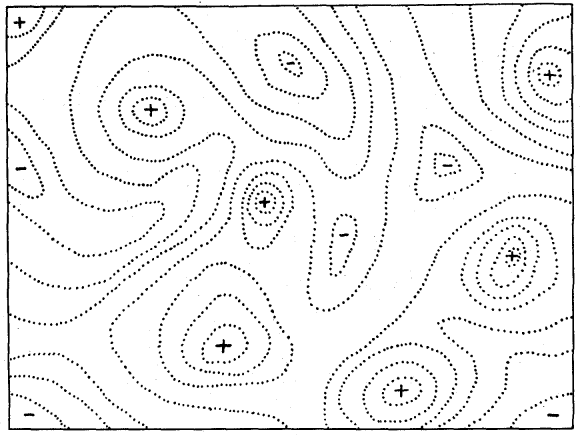
\includegraphics[scale=0.5]{figures/wright_diagram.png}
	\caption{Representación esquemática de un diagrama de Wright. Tomada de la referencia \cite{wright1932roles}}
	\label{fig:wrightDiagram}
\end{figure}

Esta representación ha sido aplicada a la descripción del destino celular a lo largo de una linea de diferenciación \cite{casey2020theory}. Sin embargo, hasta donde sabemos, no hay gráficos basados en datos reales para un tejido dado que represente al menos de forma parcial un diagrama de Wright con más de dos máximos. En el presente trabajo, mostramos un diagrama para la materia blanca del cerebro en el que el estado normal (N) se representa junto con el atractor de glioblastoma (GBM) y el máximo relacionado con la enfermedad del Alzheimer (AD).

La AD se caracteriza por la pérdida progresiva de células neuronales, mientras que el GBM es un tipo de cáncer cerebral que implica la proliferación descontrolada de células. Algunas investigaciones muestran que pacientes con la AD podrían tener un menor riesgo de desarrollar GBM. Por ejemplo, en la referencia \cite{ou2012does} muestran que ambas enfermedades presentan un aumento en el estrés oxidativo, pero en la AD, esto hace que las células neuronales sean más vulnerables a la muerte, mientras que en el GBM, las células cancerosas se vuelven más resistentes. Además, se plantea que la degeneración de células que secretan acetilcolina en la AD podría tener un efecto protector contra el cáncer, ya que esta sustancia puede estimular el crecimiento de células cancerosas.

% Ou
%Claro, aquí tienes un resumen de la relación inversa entre el Alzheimer y el glioblastoma según el artículo que estás viendo:
%
%Enfermedades Contrapuestas: El Alzheimer se caracteriza por la pérdida progresiva de células neuronales, mientras que el glioblastoma es un tipo de cáncer cerebral que implica la proliferación descontrolada de células.
%Estrés Oxidativo: Ambas enfermedades muestran un aumento en el estrés oxidativo, pero en el Alzheimer, esto hace que las células neuronales sean más vulnerables a la muerte, mientras que en el glioblastoma, las células cancerosas se vuelven más resistentes1.
%Acetilcolina: La degeneración de células que secretan acetilcolina en el Alzheimer podría tener un efecto protector contra el cáncer, ya que la acetilcolina puede estimular el crecimiento de células cancerosas.

En \cite{Driver_2012} concluyen que los sobrevivientes de cáncer tienen un riesgo 33 \% menor de desarrollar la AD en comparación con aquellos sin antecedentes de cáncer. Las personas con la AD tienen un riesgo 61 \% menor de desarrollar cáncer.

%Driver
%Claro, aquí tienes un resumen de la relación inversa entre el Alzheimer y el cáncer, según el estudio de Framingham:
%
%Riesgo reducido de Alzheimer en sobrevivientes de cáncer: Los sobrevivientes de cáncer tienen un riesgo 33% menor de desarrollar Alzheimer en comparación con aquellos sin antecedentes de cáncer.
%Menor riesgo de cáncer en pacientes con Alzheimer: Las personas con Alzheimer tienen un riesgo 61% menor de desarrollar cáncer, posiblemente debido a un diagnóstico insuficiente.
%Cánceres relacionados con el tabaco: Los sobrevivientes de cánceres relacionados con el tabaco tienen un riesgo aún menor de Alzheimer, pero un mayor riesgo de accidente cerebrovascular.
%Posibles explicaciones biológicas: La relación inversa podría deberse a mecanismos biológicos compartidos entre el cáncer y las enfermedades neurodegenerativas, como la regulación de la apoptosis y la proteína Pin1.


%roe2009
%Claro, aquí tienes un resumen de la relación entre el Alzheimer y el glioblastoma según el artículo:
%
%Reducción del riesgo: La presencia de Alzheimer (AD) se asocia con un riesgo reducido de hospitalización por cáncer, incluyendo glioblastoma.
%Mecanismos comunes: Se sugiere que mecanismos moleculares comunes podrían estar involucrados en ambas enfermedades, regulando la muerte y supervivencia celular.
%Estudios previos: Otros estudios han mostrado asociaciones similares entre el cáncer y enfermedades neurodegenerativas como el Parkinson.
%Diferencias raciales: La relación entre el cáncer y el Alzheimer varía según la raza, con efectos opuestos observados en minorías, aunque los datos no son concluyentes debido al tamaño de muestra pequeño.


%musicco
%Claro, aquí tienes un resumen del artículo sobre la relación inversa entre el Alzheimer y el cáncer:
%
%Objetivo del estudio: Evaluar la incidencia de cáncer en personas con Alzheimer y la incidencia de Alzheimer en personas con cáncer1.
%Resultados principales: El riesgo de cáncer en pacientes con Alzheimer se redujo a la mitad, y el riesgo de Alzheimer en pacientes con cáncer se redujo en un 35%2.
%Conclusión: Existe una relación inversa entre el Alzheimer y el cáncer, sugiriendo que ambos podrían ser manifestaciones opuestas del envejecimiento.
%
%\alert{El trabajo presentado como tesis de diploma consta de una introducción, tres capítulos,las conclusiones y las recomendaciones. El contenido se distribuye de la siguiente forma:}

\begin{itemize}
	\item[$\bullet$] \textbf{Introducción:}
	
	\item[$\bullet$] \textbf{Capítulo 1:} 
	
	\item[$\bullet$] \textbf{Capítulo 2:} 
	
	\item[$\bullet$] \textbf{Capítulo 3:} 
	
	\item[$\bullet$] \textbf{Conclusiones:} 
	
	\item[$\bullet$] \textbf{Recomendaciones:} 
	
	
\end{itemize}